\vspace*{-5mm}
\mysection{Architectural Design}

\mysubsection{Overview}
In this chapter we will analyze the proposed architecture and components of Travlendar+ system.\par
The proposed architecture is composed by three tiers :
\begin{itemize}
	\setlength{\leftskip}{0.5cm}
	\item \emph{Presentation Tier : }it's represented by the Browser and the Mobile App, the View part of our system.
	\item \emph{Web and Business Tier : }it's represented by the Web Server, which responds to the user's HTTP requests, and the Application Server, which contains all the Business Logic.
	\item \emph{Database Tier : }it's represented by the DB Server, that contains and manages persistent data in an efficient way.
\end{itemize}
\begin{figure}[H]
	\centering
	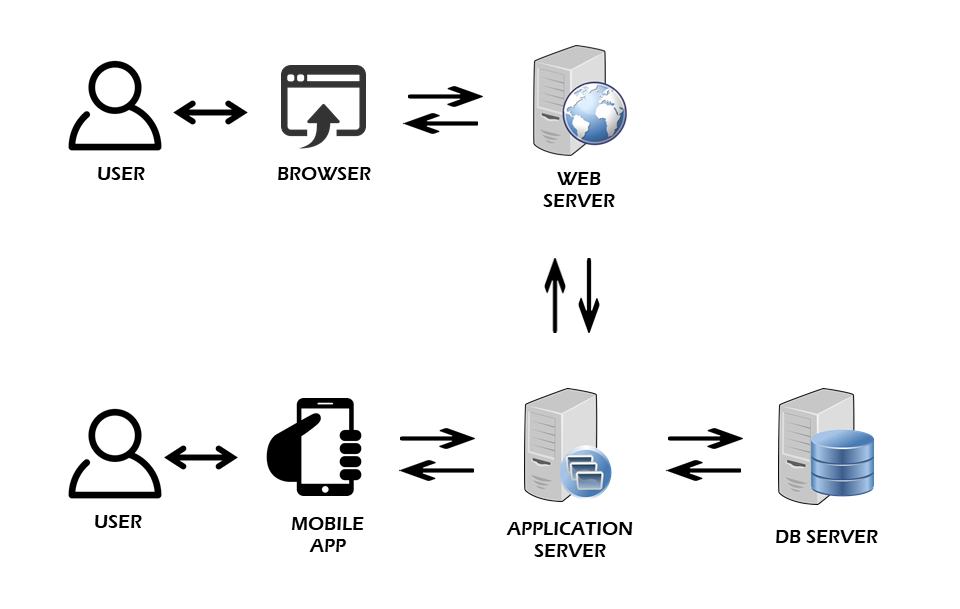
\includegraphics[scale=0.35]{Images/Architecture/Proposed_Architecture}
	\caption{Proposed Architecture}
\end{figure}

\mysubsection{High Level Components and Their Interactions}
\begin{figure}[H]
	\centering
	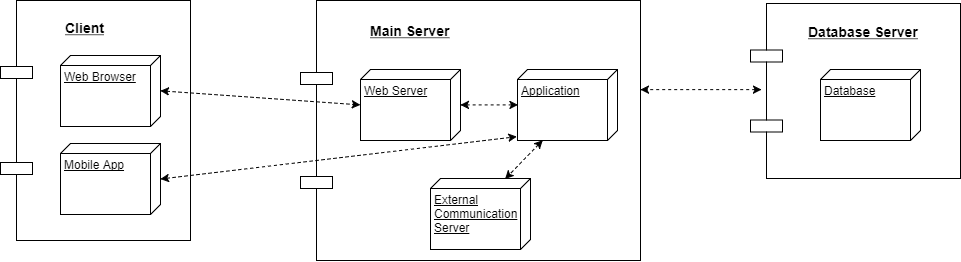
\includegraphics[scale=0.35]{Images/Architecture/Components_High_Level}
	\caption{Components High Level}
\end{figure}

The system is divided in three main layers: Presentation Layer, Business Layer and Data Layer.
The presentation layer is both a web-based application and a mobile application. For the web application we will have a very thin client with the only aim of performing requests, through a web server, to the Business layer and receiving the HTML pages with the demanded information.
On the other hand, the mobile application will not require an interface with the web server because it will communicate directly with the server.

The main server is composed by three parts : the Web Server, mentioned here above, the Application and the External Communication Server. The application part of the main server contains all the system's logic: it receives requestes and input data from the client side and performs all the necessary operations.
The External Communication Server part is in charge to handle all the comunication with the external services to retrieve data of interests from other systems in order to achieve the system goals.
Our system, being a calendar based application, will have the main issue of managing a richly structured body of information. In our case, this information will be persistently stored in multiple Data Bases, each one containing a precise schema with a precise kind of data, and they always have to reflect the true state of affairs. For this reason, every client request, implicating a changing data operation is preceded by a set of controls performed by the Business logic in order to maintain the database’s consistency.

\mysubsection{Component View}
\begin{figure}[H]
	\centering
	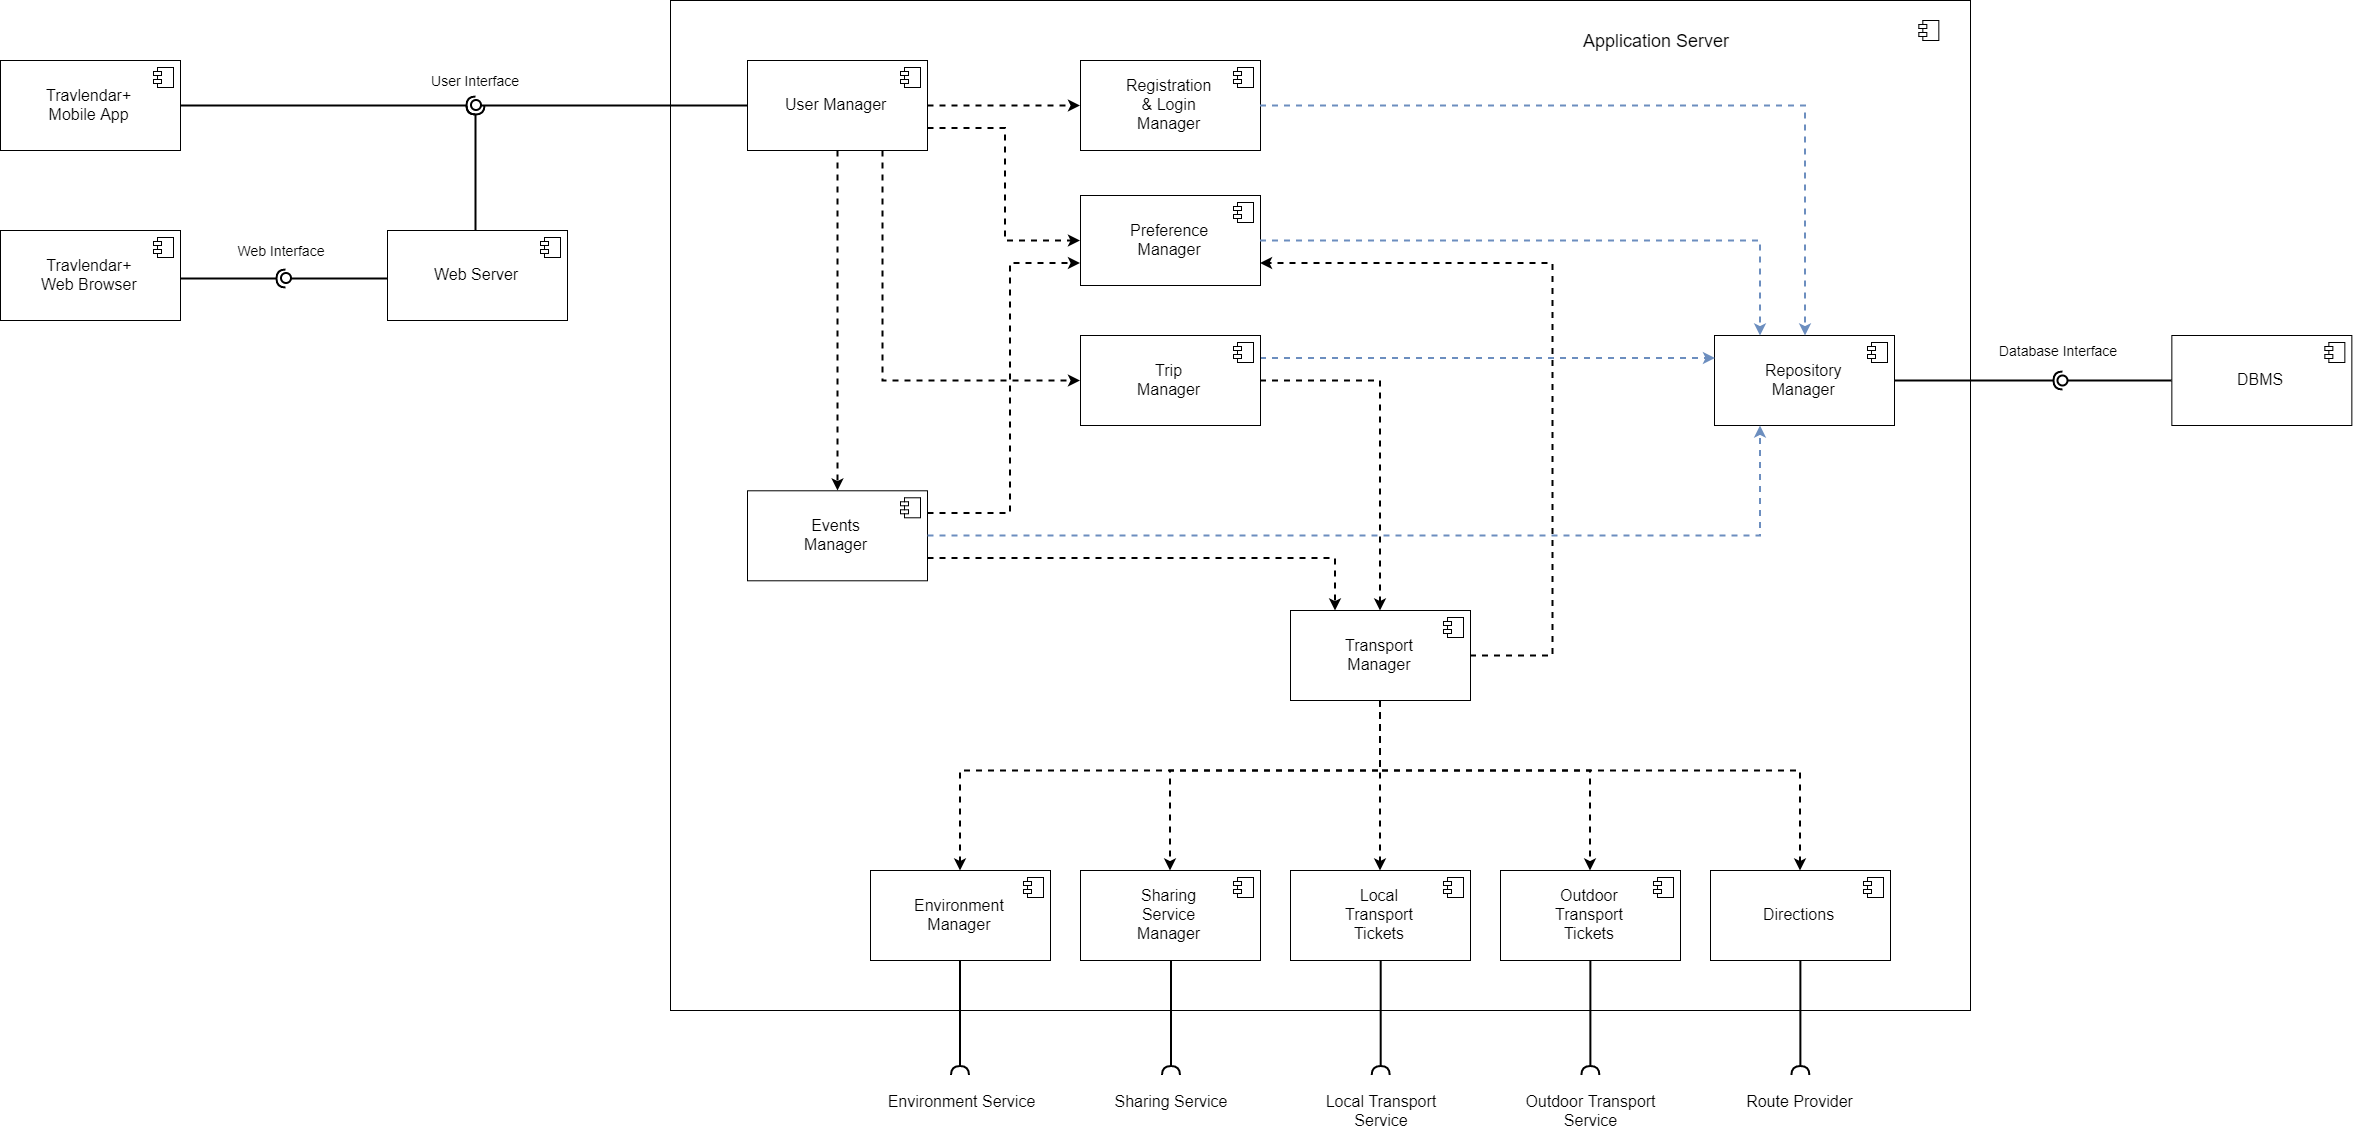
\includegraphics[scale=0.17]{Images/Architecture/Components_View}
	\caption{Component View}
\end{figure}
\mysubsubsection{Travlendar+ Mobile App}
This is the component responsible for the communication between user devices, i.e. smartphone, and the rest of the system. It will exchange REST messages with the \emph{userInterface} and render based on the server replies.\par
In order to communicate with the server the component will use specific frameworks and libraries depending on the specific device used by the user (i.e. Android SDK Platform for Android smartphones).\par
This component represents the View part of our MVC pattern.

\mysubsubsection{Travlendar+ Web Browser}
This is the component responsible for the communication between user's browser and the rest of the system.\par
It sends HTTP requests to the \emph{webInterface} in order to get back from the server HTML pages and static resources like CSS and JavaScript files.

\mysubsubsection{Web Server}
This component is responsible for the HTTP responses of the \emph{webInterface}. Its main function it’s to elaborate pages, generate contents in a very dynamic way and send them to the browser. These processes are performed by the Web Server instead of the user's Browser for managing in the most efficient way the user CPU's load.\par
An example could be the Apache HTTP Server. It’s cross-platform, highly scalable and use a \emph{gzip} module to reduce web pages size (weight).

\mysubsubsection{User Manager}
This is one of the most important component of the server because it handles the communication with the user, so it takes care of all possible breakouts or errors that may occur runtime. It also manages all user’s request redirecting them to other server’s specific components.

\mysubsubsection{Registration \& Login}
It allows user to register and login to the system memorizing and verifying user’s credentials.

\mysubsubsection{Preference Manager}
It allows user to set all his preferences such as carbon footprint, TAGs, residence location, etc… So its aim is to memorize these preferences’ data in the DB through the Repository Manager and get them every time is needed.

\mysubsubsection{Trip Manager}
This component handles all user’s trips, allowing him to add, delete or edit trips. It allows also the user to buy tickets to reach the trip’s location (through the Outdoor Transport Tickets component) and tickets to use the local transport service in the destination city (through the Local Transport Tickets).

\mysubsubsection{Events Manager}
This component takes care of user’s calendar managing the events that the user wants to add, delete, edit or visualize.\par
So every time he wants to :
\begin{itemize}
	\setlength{\leftskip}{1cm}
	\item \emph{insert or edit an event}, this component will check through the Repository Manager if in the DB there is an overlap and if the event is reachable from the previous one (using also Transport Manager to verify route’s time).
	\item \emph{delete an event}, this component will simply delete it in the DB.
	\item \emph{visualize an event}, this component will check through the Transport Manager the available means of transport, the time needed and the route to reach the event.
\end{itemize}

\mysubsubsection{Transport Manager}
This component handles all event’s means of transport and tickets. About transport, it filters the means according to :
\begin{itemize}
	\setlength{\leftskip}{1cm}
	\item the means selected in the event’s TAG;
	\item the $CO_2$ preference;
	\item the means selected in the “Available Means” in Preferences;
	\item the means available to reach the event (received by the route provider);
	\item the weather conditions;
	\item the strikes.
\end{itemize}
It allows also to buy local transport tickets if the user needs to. 

\mysubsubsection{Directions}
This component handles the communication with the route provider in order to get maps, means and routes to reach a specific destination. To get these information it uses API requests (an example are Google APIs).
It also parses and elaborates the API responses in specific structures in order to allow the other server’s components to use them in the best way.

\mysubsubsection{Environment Manager}
This component is used by our system to check and warn the user about the weather's conditions and the transport strikes.
It uses API requests in oreder to communicate with the external services.

\mysubsubsection{Sharing Service Manager}
This component allows our server to communicate with external sharing services in order to get the nearest sharing mean of transport's location.

\mysubsubsection{Local Transport Tickets}
It takes care of the communication with the local transport services for getting information about the available tickets, suggesting to the user the best one to buy based on his travel's needs.

\mysubsubsection{Outdoor Transport Tickets}
It takes care of the communication with the outdoor transport services in order get information about the available tickets and means of transport.

\mysubsection{Deployment View}
\textcolor{red}{\Huge INSERISCI TESTO}
\begin{figure}[H]
	\centering
	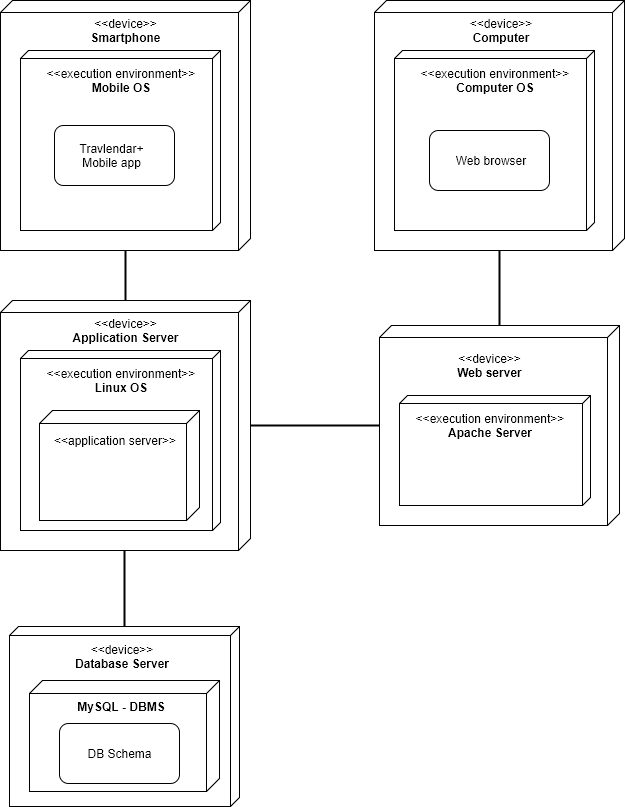
\includegraphics[scale=0.17]{Images/Architecture/Deployment_View}
	\caption{Deployment\_View}
\end{figure}

\mysubsection{DB Structure}

INSERT DBMS DIAGRAM

\mysubsection{Runtime View}
In this section we will see some Runtime Views in order to see how the components interact according to specific requests.
Because of this we decide to consider for the client-side just the Web Browser, in order to see the interaction between the Browser and the Web Server and the Web Server and the Application Server's components.

\mysubsubsection{Registration}
This Runtime View shows a user's Registration process.\par
First of all the Web Server sends to the user the registration\_form to fulfil with his credentials. Then, once it receives the form, it sends to the Server the inserted information.\par
Now it’s important to check if the email is already used for another account or not. So, in order to do that, the server asks the DBMS to search for it and get it. If the get\_result it’s equal \emph{Null} it means that the email it’s not used, so the server can complete the registration saving in the DB the user’s credentials. Otherwise, the server will notify the user that the inserted email can’t be used.
\begin{figure}[H]
	\centering
	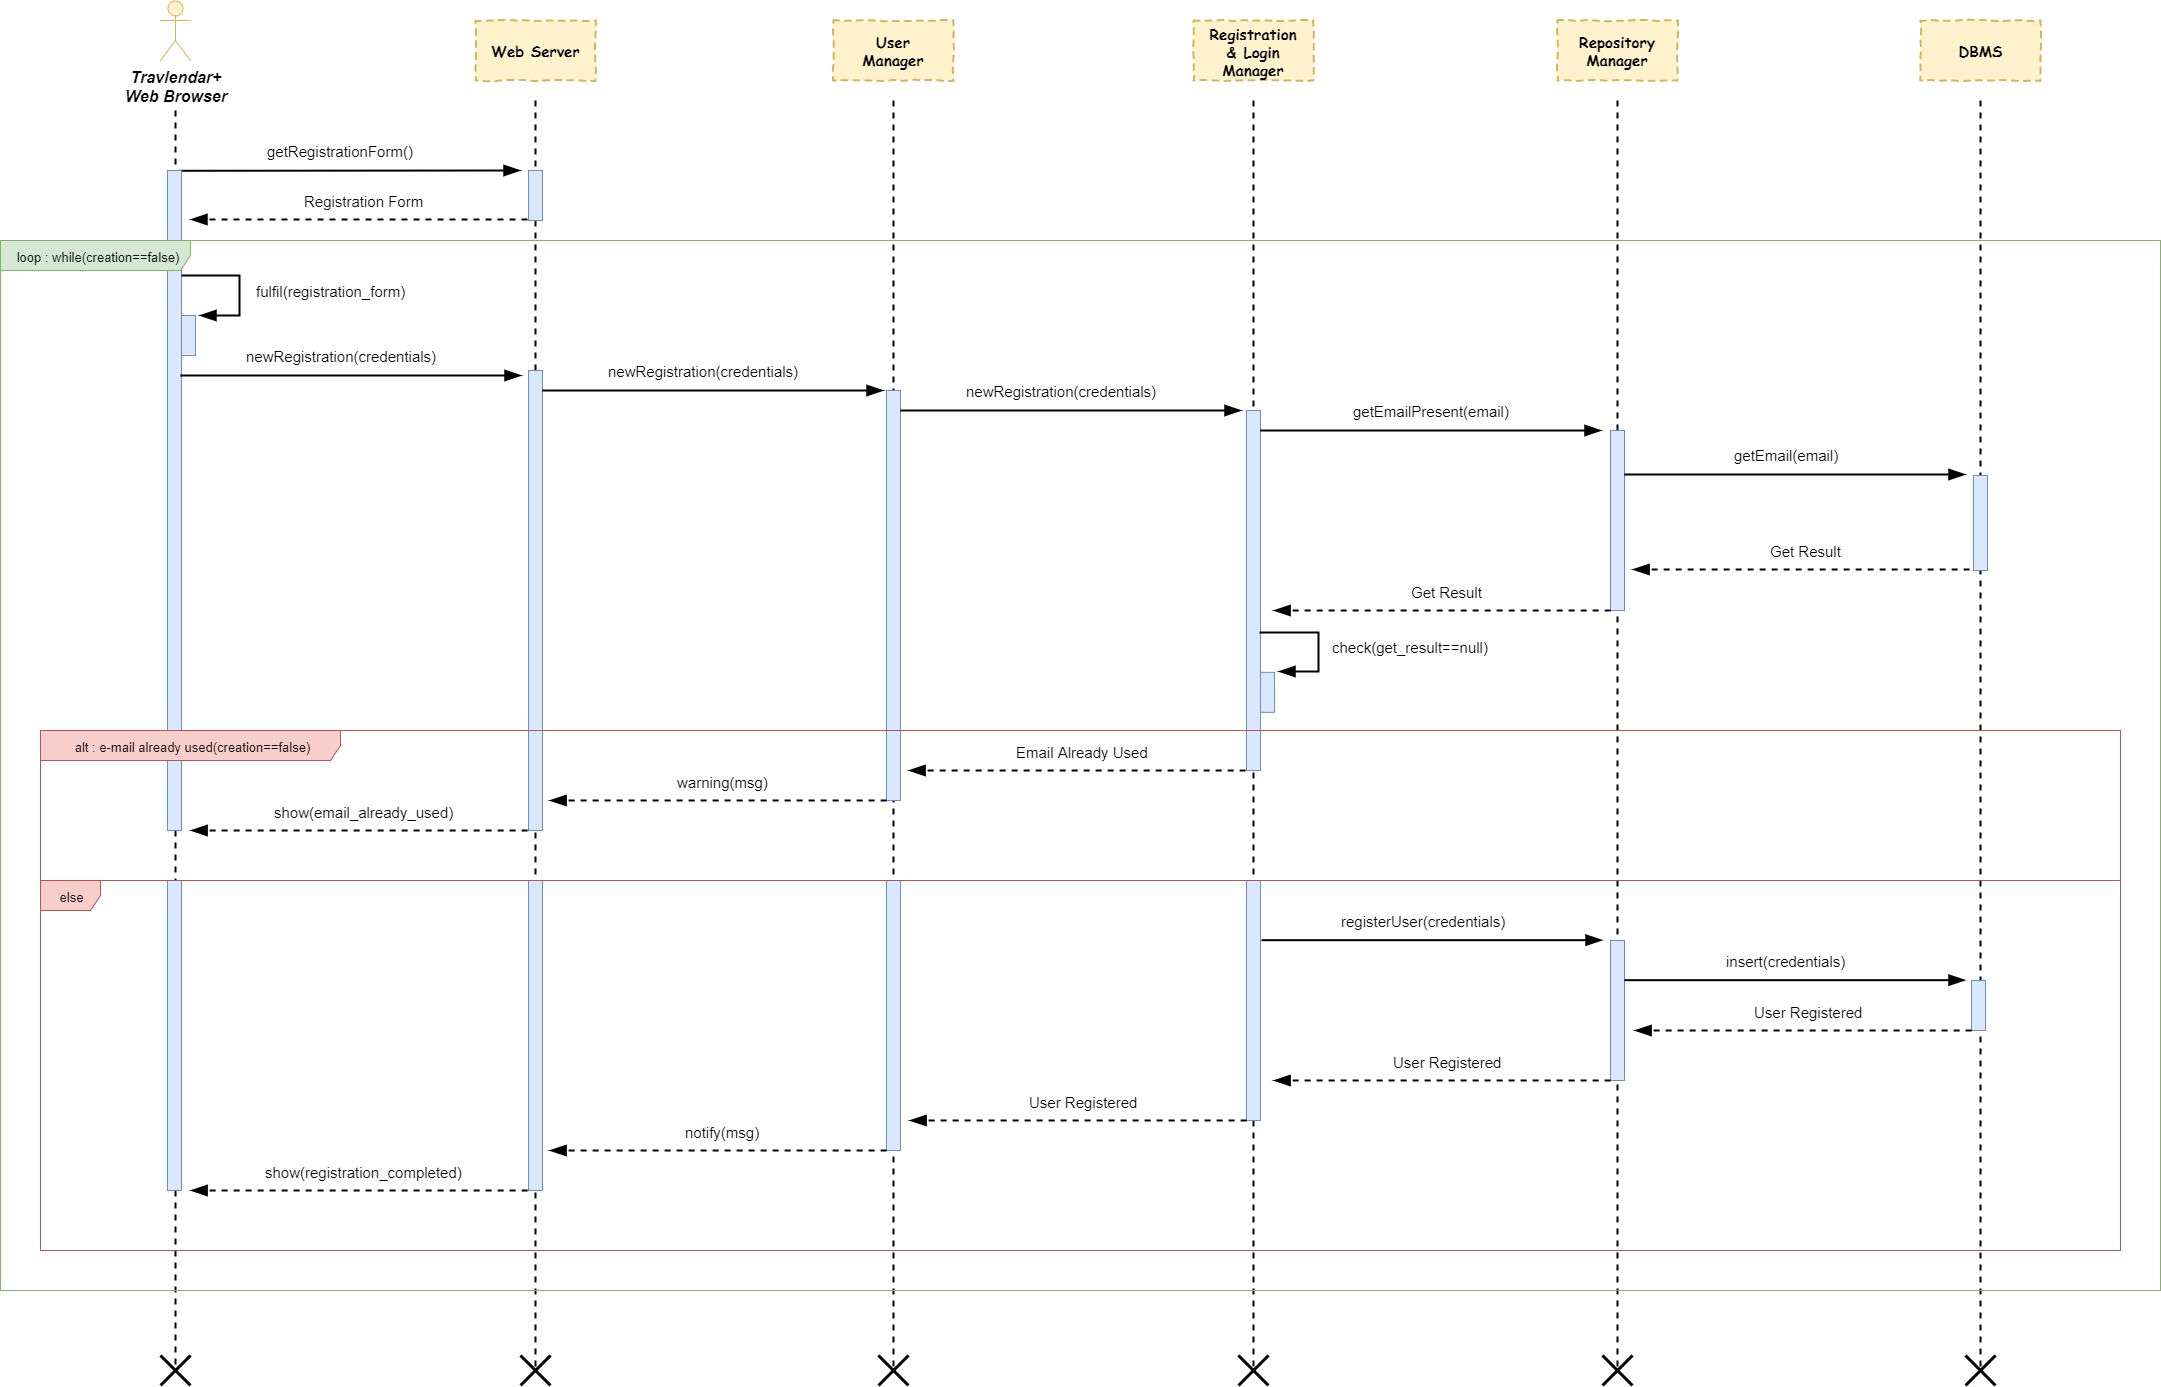
\includegraphics[scale=0.2]{Images/Runtime/Registration}
	\caption{Registration Runtime View}
\end{figure}

\mysubsubsection{Login}
This Runtime View shows a user's Login process.\par
Like the previous runtime, the Web Server sends to the user the login\_form to fulfil with his credentials. Once he receives that, it sends the inserted information to the server, which now has to make some checks.\par
First of all it has to check if the user’s email is saved in the DB and next if the user’s password is correct. So, in order to do that in an efficient way, the server asks the DBMS to get him the password related to the inserted email. This means that if the get\_result is equal \emph{Null} then there is no account registered with that email. Otherwise, the server, more specifically the Registration \& Login Manager, has to check if the get\_result is equal to the inserted password.
If that check succeeds then the user is logged and the server gets from the DB the events related to the current month and shows them to the client.
\begin{figure}[H]
	\centering
	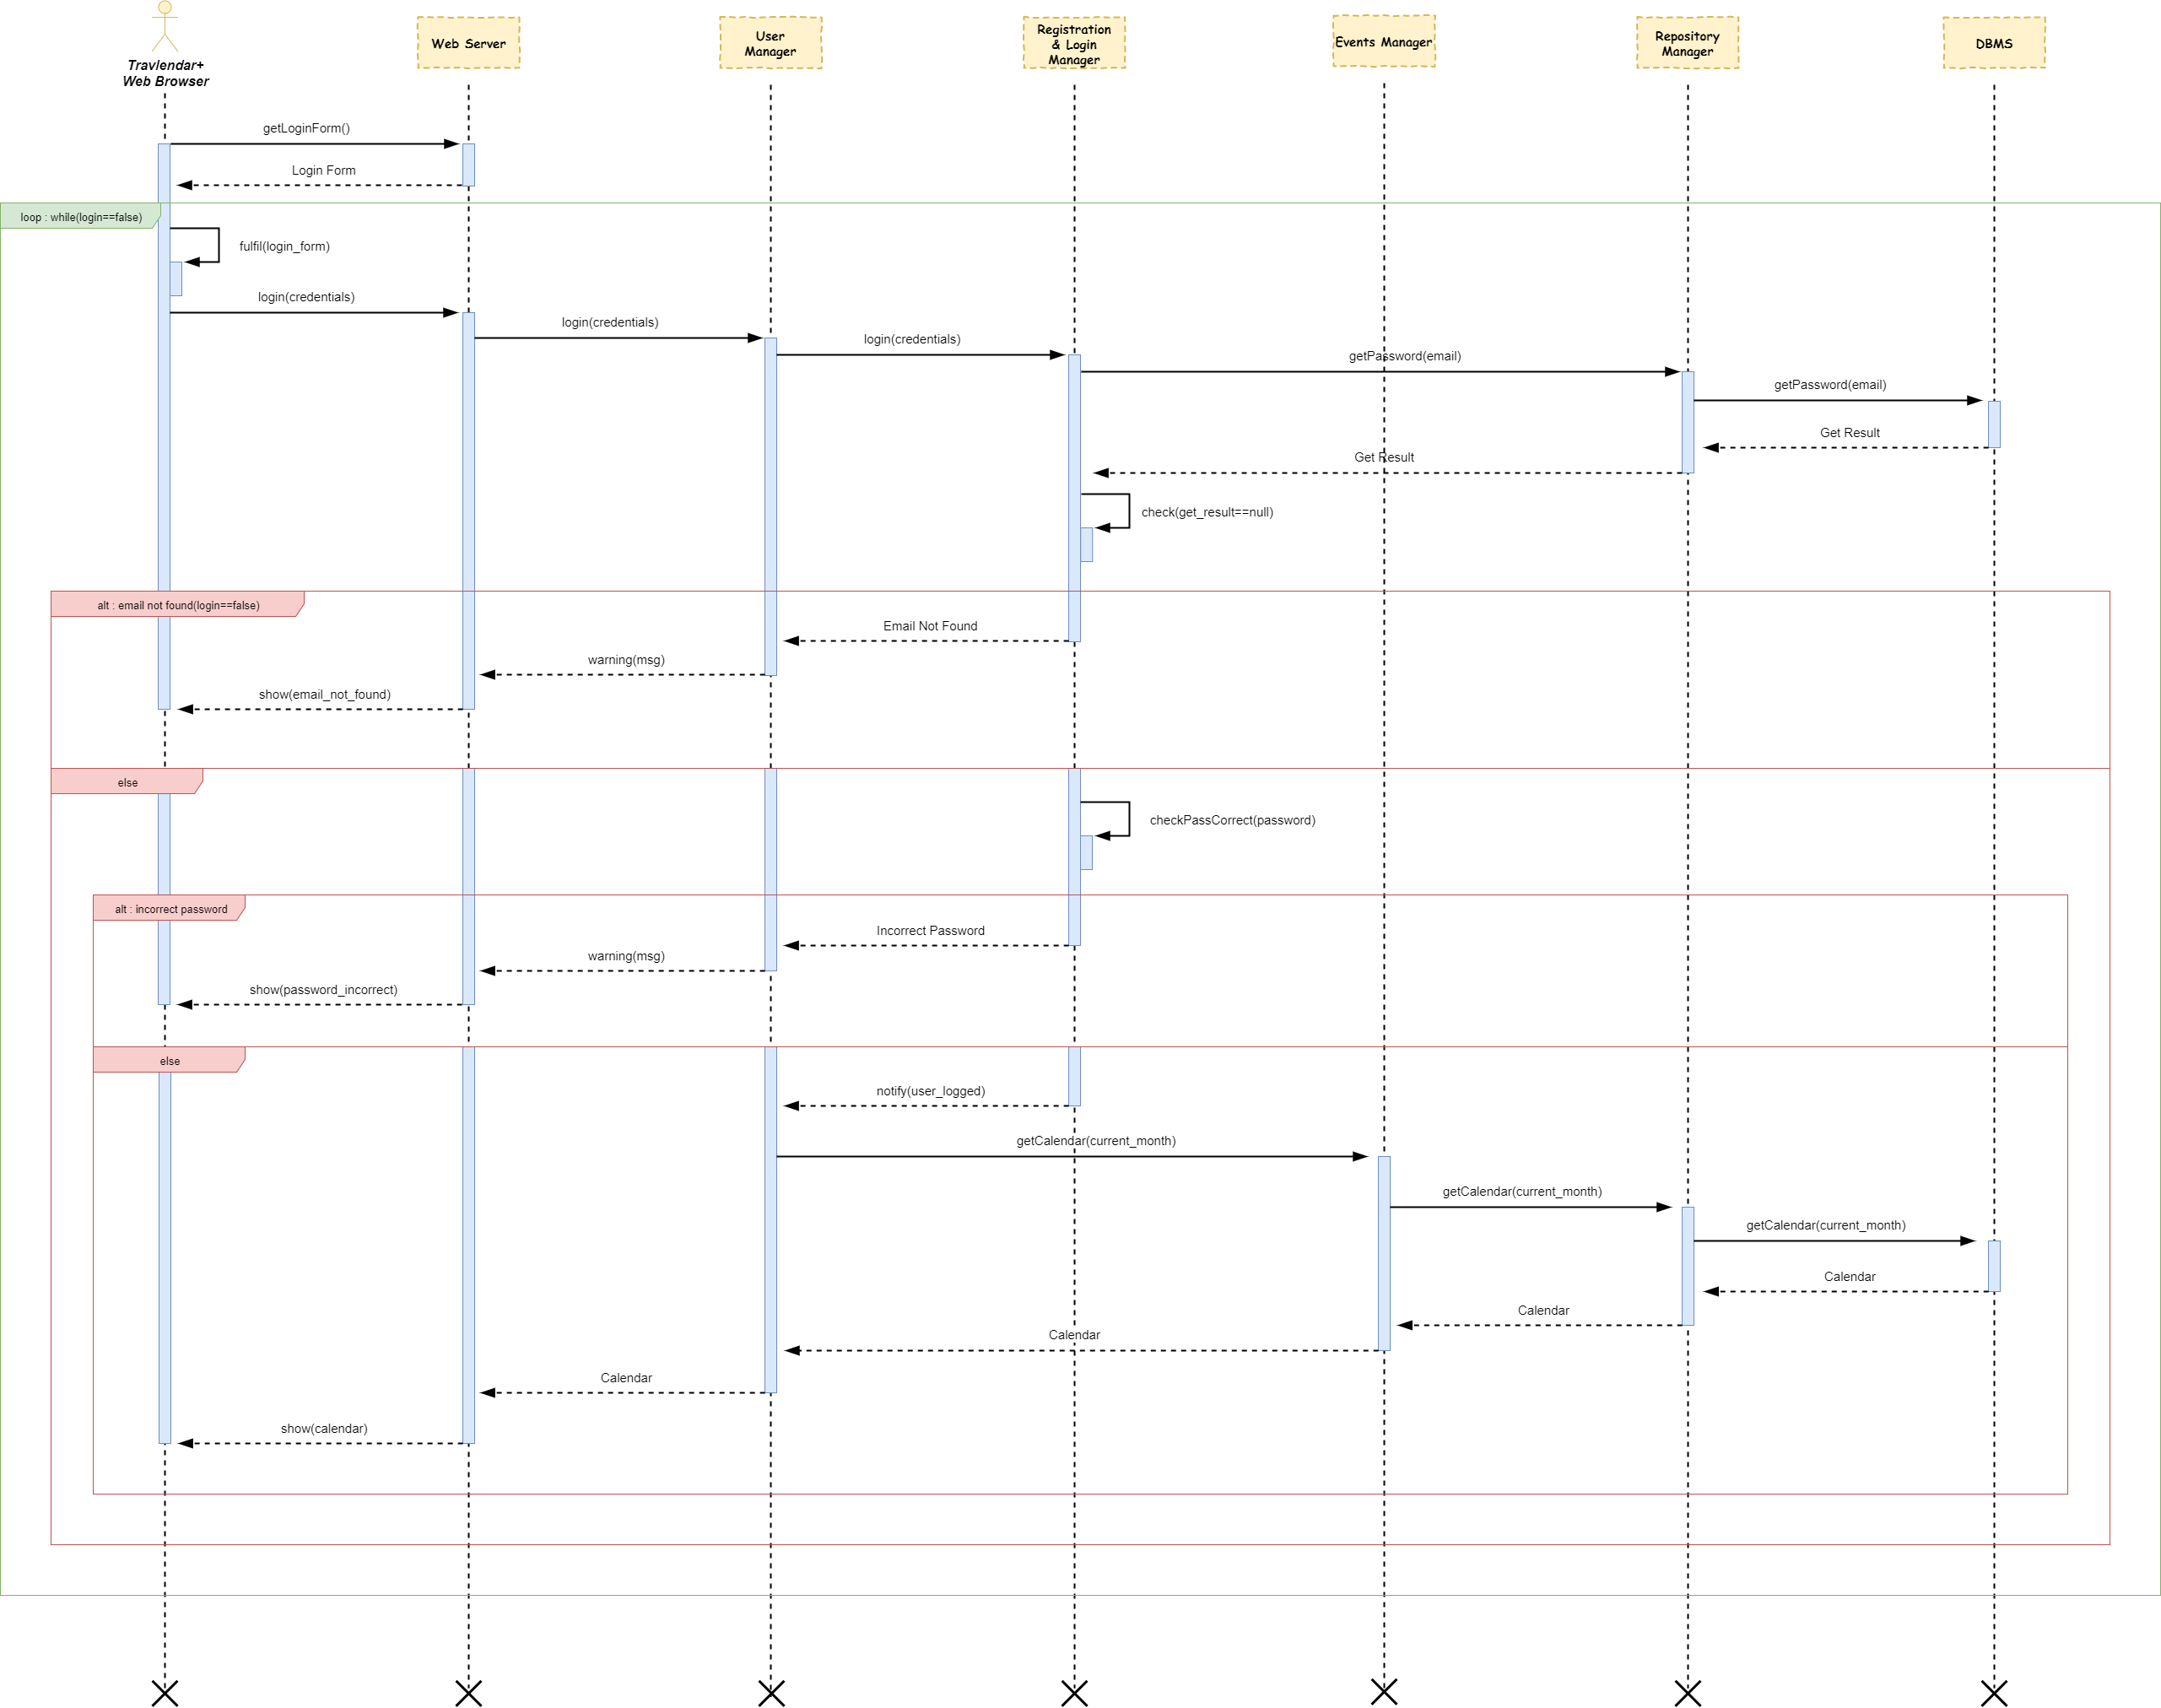
\includegraphics[scale=0.17]{Images/Runtime/Login}
	\caption{Login Runtime View}
\end{figure}

\mysubsubsection{Add Event}
This Runtime View shows the AddEvent process.
In order to reduce the diagram size we make some premises :
\begin{itemize}
	\setlength{\leftskip}{1cm}
	\item There is a Previous and a Next Event, before and after the event that the user is adding. In this way we don’t have to put in the runtime the check that verifies if the getPreviousEvent() or the getNextEvent() is equal to Null.
	\item The user hasn’t already configure the lunch preference, so there is no lunch event in the calendar. In this way we don’t put the check that, in the case that the inserted event overlaps with another one, verifies if the existing event is a Lunch. If it’s a Lunch the system has to check if it can be moved or reduced.
\end{itemize}
Even in this runtime the user first of all has to complete the event\_form and send it to the server.
Once Events Manager receives the data it has to check :
\begin{enumerate}
	\setlength{\leftskip}{1cm}
	\item \emph{If the event Overlaps :} Events Manager asks the Repository Manager to search in the DB if there’s a planned event at the same time of the inserted one. If the get\_result it’s equal to \emph{Null} it means that there’s no overlap.
	\item \emph{If the event is reachable from the previous one :} Events Manager asks the Repository Manager to get the information of the previous event, especially its location. Once received, it sends both locations to the Directions Component in order to get the route’s time, so it can check finally if the event is reachable or not.
	\item \emph{If the next event is reachable from the inserted one :} it’s like the previous check but instead of getting the information from the DB of the previous event, it gets the one of the next event.
	If all checks succeed, the server adds the event in the DB and show it to the user.
\end{enumerate}
\begin{figure}[H]
	\centering
	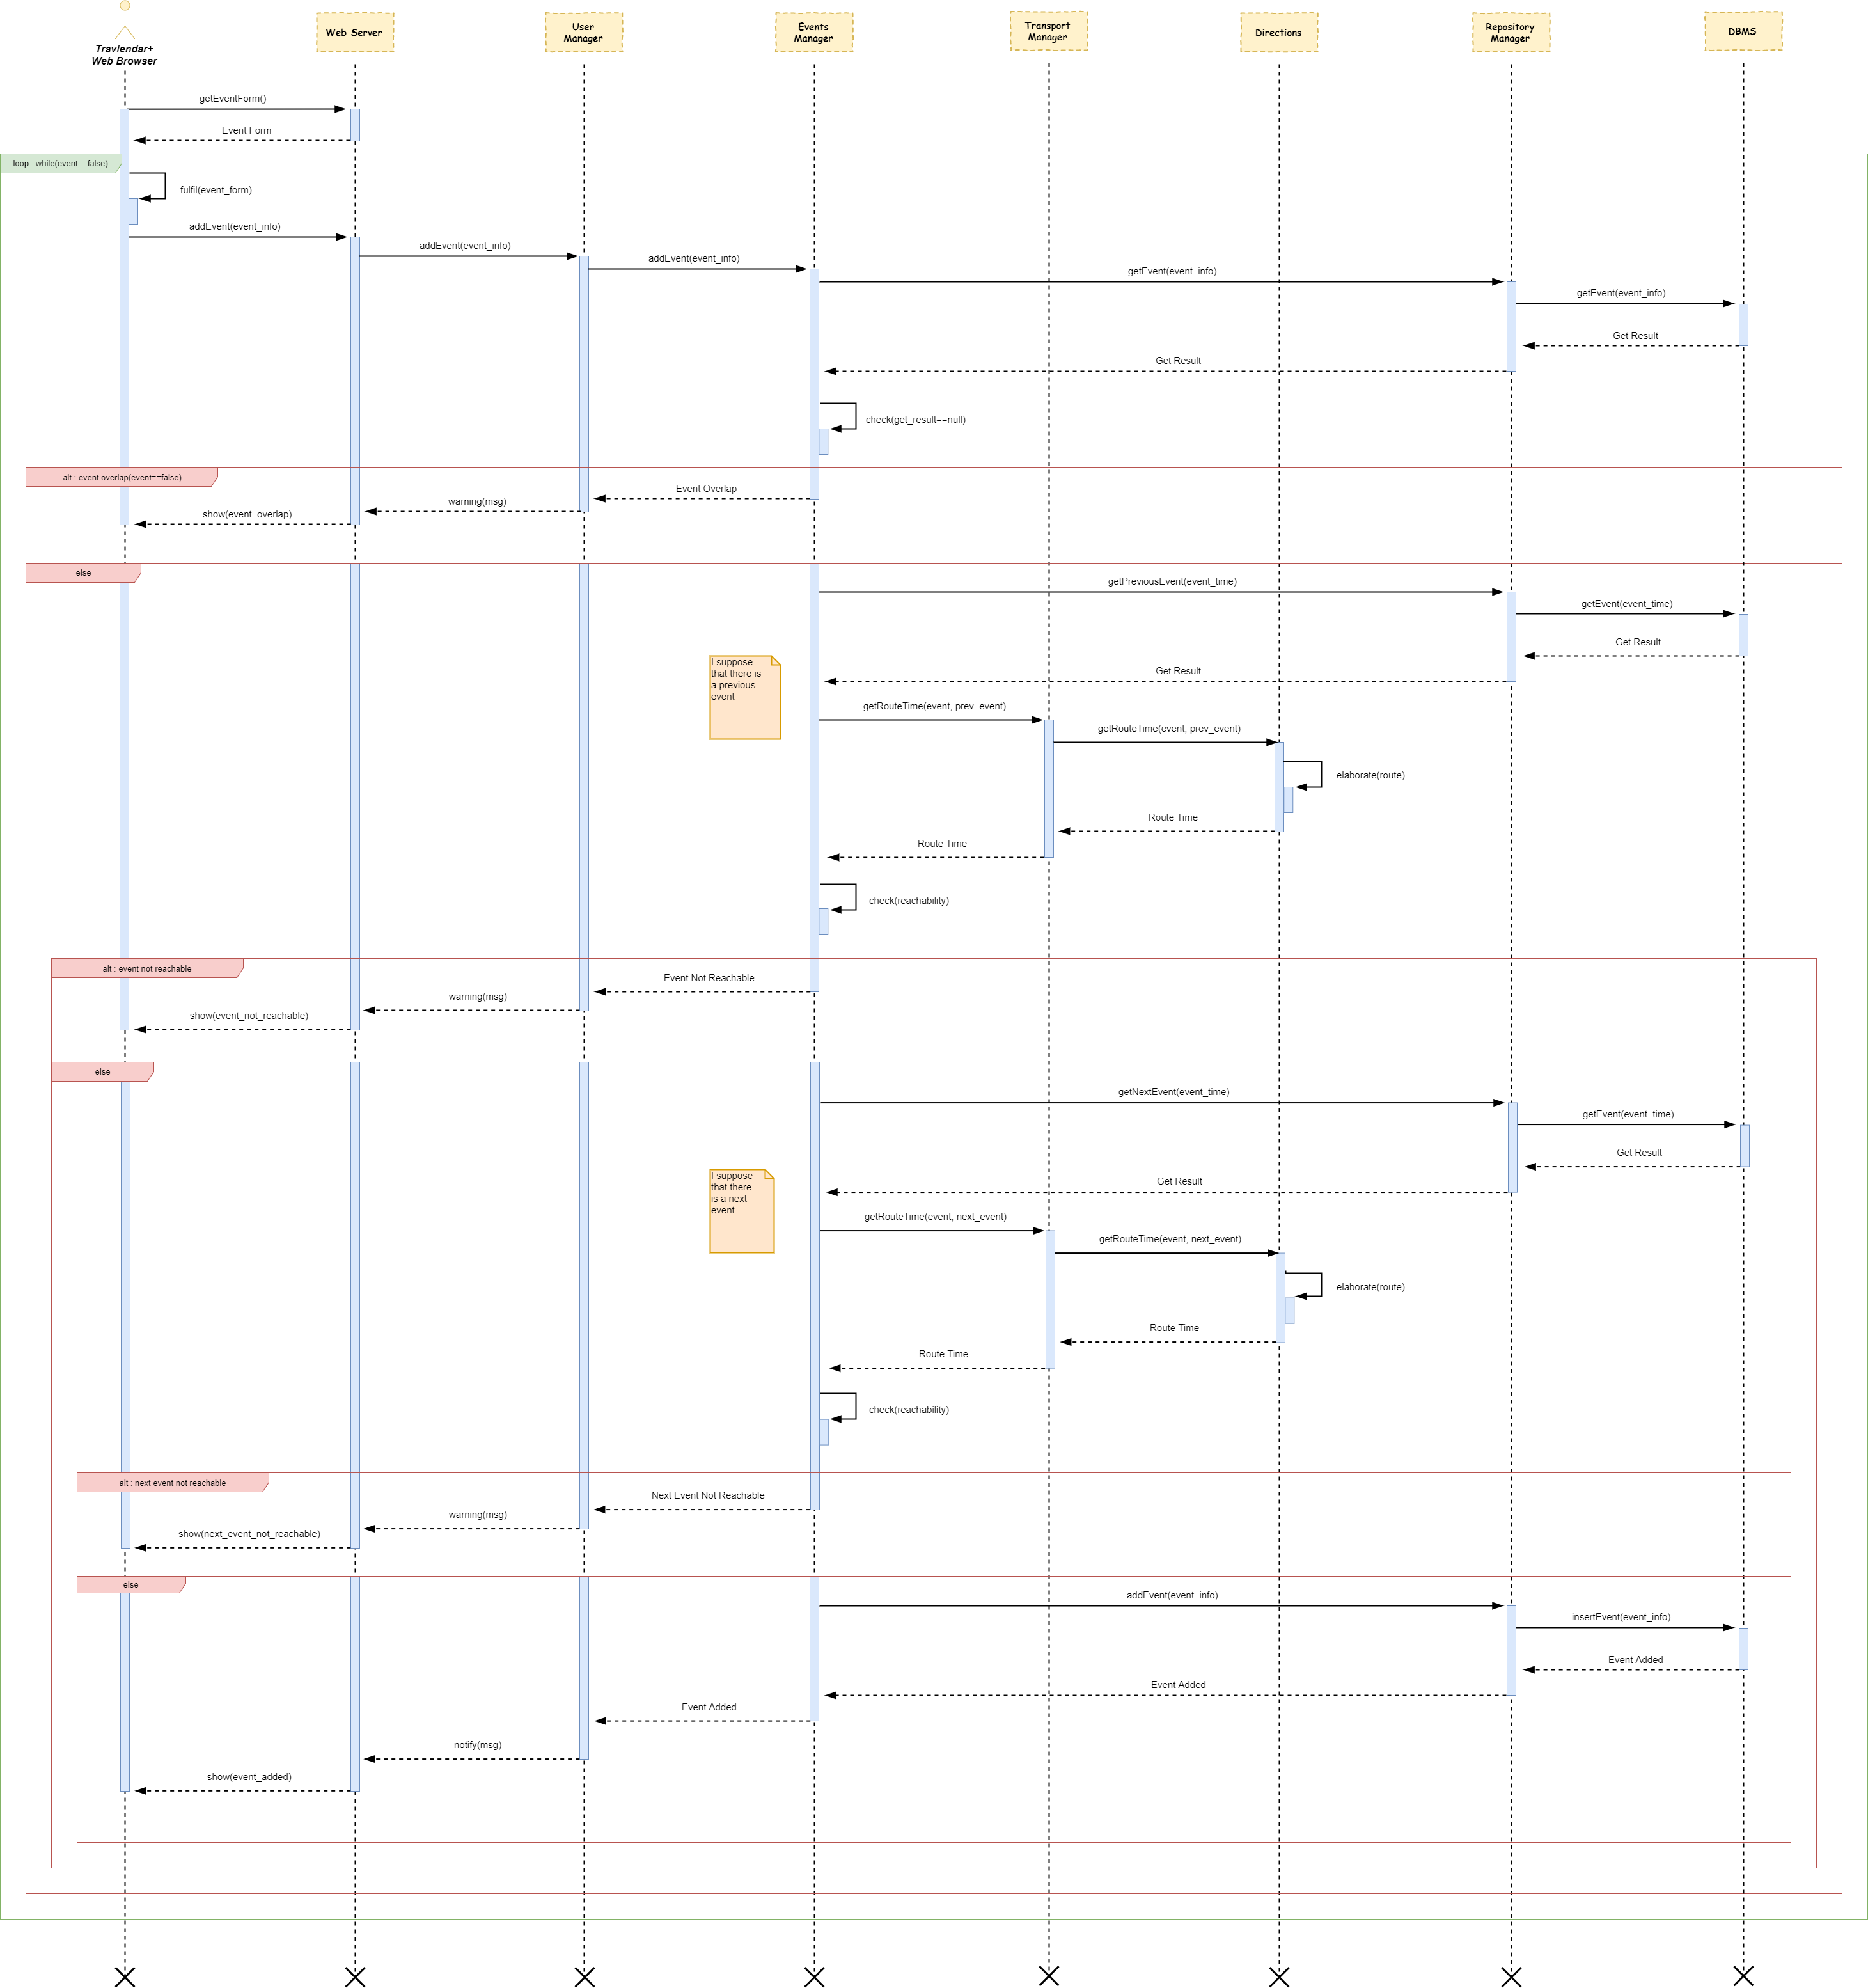
\includegraphics[scale=0.15]{Images/Runtime/Add_Event}
	\caption{Add Event Runtime View}
\end{figure}

\mysubsection{Selected Architectural Styles and Patterns}
Our system architecture proves to be a mix between three well known architectural styles, in particular : 

\begin{itemize}
\setlength{\leftskip}{0.5cm}
\item \emph{Client/Server Architectural style}
\item \emph{Main program with subroutines architectural style}
\item \emph{Service oriented Architectural style}
\item \emph{Event Based Architectural style}
\end{itemize}

Travlendar+ is both a web-based application and a mobile application. For the web application we will have a very thin client with the only aim of performing requests to the Business Logic through a web server.
On the other hand, the mobile application will not require an interface with the web server because it will communicate directly with the server.
\\\par
The main server will contain all the logic of the system. The main component of the logic will be the User manager. This component will perform as the Main program in the \emph{Main program with subroutines style}: it will receive the requests from the clients and call the right sub-components for accomplishing the goals related to the request.
\\\par
An essential our system business, as said in the RASD, will be to provide directions related to the precise travel means, sharing means’ position and give tickets information about local and outdoor public transport. All these information will not be stored in our DBs, but they will be retrieved with API REST requests to appropiate external services. For this goal we will use a \emph{SOA style}. 
In our system we will have a component called Transport manager that will be able to distinguish the kind of the request and demand the aim of submitting it to the right external service to another precise component devoted to a certain type of external services connections. Once received the information, their manipulation will be performed internally to the business logic of the system. In these way we will have the possibility of adding new components for incoming kind of transportation, also personalized, in a very simple and scalable way.
\\\par
The last style exploited is the \emph{Event based Architectural style}, and it is used for the notification system that will be always attending particular events that, if happens, triggers a notification that is immediately sent to the right clients subscribed to the topic. 

\mysubsection{Design patterns}

\mysubsubsection{MVC}
\begin{figure}[H]
	\centering
	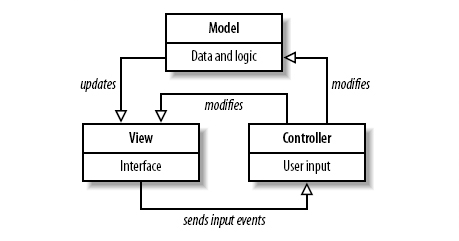
\includegraphics[scale=0.4]{Images/Patterns/MVC_Pattern}
	\caption{MVC Pattern}
\end{figure}
The Database server contains all the software’s data and constitutes the model part. The presentation layer with the web-based application and the mobile application is the view that is released to the user. Finally the main server,  that is the business logic layer, it’s the control part.

\mysubsubsection{Observer}
\begin{figure}[H]
	\centering
	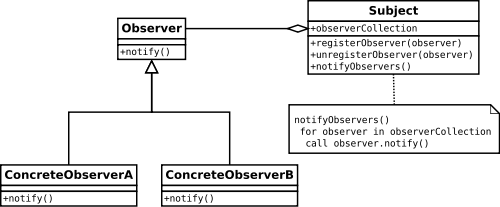
\includegraphics[scale=0.45]{Images/Patterns/Observer_Pattern}
	\caption{Observer Pattern}
\end{figure}
Our software has to be able to advise the user that he has to take a certain mean of transport in a specific time for arriving on time, or that the registered season ticket is expiring or also the possibility of a strike or a bad meteorological condition. All these events have to be supported by a notification system.These needs will be implemented with this pattern.  There will be a specific group of event listener, namely objects that extend a common abstract class. The system will have as much kind of event listener as is necessary and they could be added freely for future expansion. When during a process a state of interest for a listener is changed some checks are performed and, under some particular conditions, a notification is created and sent to the user. 

\mysubsubsection{Strategy}
\begin{figure}[H]
	\centering
	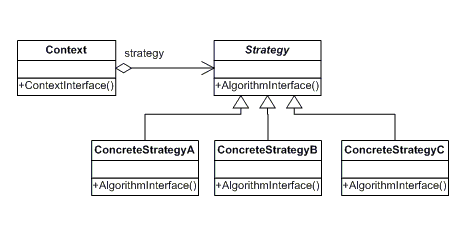
\includegraphics[scale=0.7]{Images/Patterns/Strategy_Pattern}
	\caption{Strategy Pattern}
\end{figure}
The filters applied on the data for showing particular results based on the user’s choices, for example for advising the best means of transport for a destination, will be implemented with a strategy pattern. The class that will put in order the results will have an instance of an abstract class that will be implemented by some concrete classes representing different ordering strategy. In this way the system will be able to adapt his strategy runtime and it will be very simple to add new strategy creating new classes that will implement the abstract strategy class previous mentioned.

\mysubsubsection{Composite}
\begin{figure}[H]
	\centering
	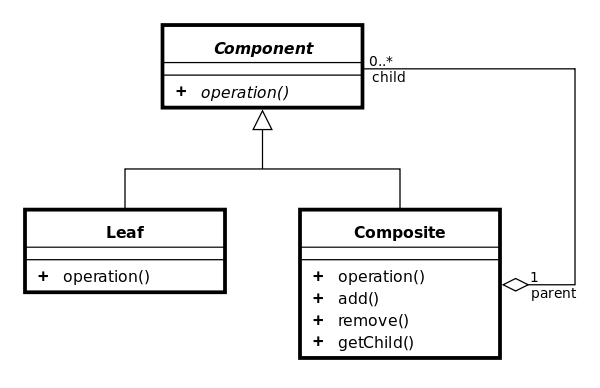
\includegraphics[scale=0.35]{Images/Patterns/Composite_Pattern}
	\caption{Composite Pattern}
\end{figure}
We will use this pattern in our system for performing in a cleaned and elegant way the various check that will have to be apply on the user input. There will be a abstract class Checker that will be extended by Composite checkers and Checkers. Each composite checker contains one or more checkers and both implements a common interface with the method \emph{check}. The class that will have to manage a specific user input will have one or more composite checkers.
When a method that have to process the user input data for passing them to an external service or to another component that will insert such a data in a DB, the check method of all the composite checker in such a class will be called and each composite checkers will recursively call his checker’s check method. In this way all the check will be applied and if something is wrong, the subsequent operation will not be executed and all the possible problems linked with that will be avoided. 
Thanks to this pattern is possible to create new checkers/composite checkers very easily and deal with complex and composite check that will be needed in future software expansions.

\mysubsubsection{Façade}
\begin{figure}[H]
	\centering
	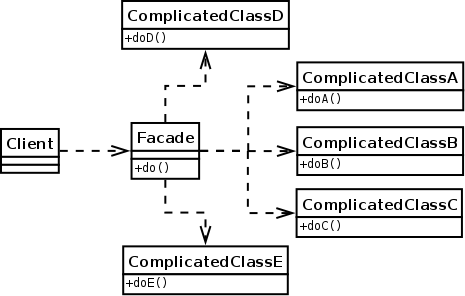
\includegraphics[scale=0.3]{Images/Patterns/Facade_Pattern}
	\caption{Facade Pattern}
\end{figure}
As guideline of our implementation, for all the complex operations that will require multiple method’s calls from different classes we will use a façade pattern. In this way we will able to hide a complex logic operation within a single method’s call. In this way we will simplify the software maintenance for future changing needs.
